% !TEX root = ../ejemplo-memoria.tex
\section{Implementación del backend}

\subsection{Herramientas, frameworks y lenguajes utilizados}

El backend de la aplicación se ha desarrollado utilizando el framework \textbf{Django} (versión 5.2.2) junto con \textbf{Django REST Framework} para la construcción de la API. Django facilita la definición de modelos, la gestión de usuarios y la exposición de endpoints RESTful de manera segura y eficiente.

Para la persistencia de datos se ha empleado \textbf{PostgreSQL} como sistema gestor de bases de datos relacional. El entorno de desarrollo y despliegue se ha gestionado mediante \textbf{Docker} y \textbf{Docker Compose}, lo que permite la portabilidad y la replicabilidad del entorno en diferentes máquinas.

Las principales herramientas y librerías utilizadas son:
\begin{itemize}
    \item \textbf{Python 3.10}
    \item \textbf{Django 5.2.2} 
    \item \textbf{Django REST Framework} (\texttt{djangorestframework})
    \item \textbf{Docker} y \textbf{Docker Compose} para la gestión de contenedores
    \item \texttt{psycopg2-binary} para la conexión con PostgreSQL
    \item \texttt{django-cors-headers} para permitir peticiones desde el frontend
    \item \texttt{Pillow} para el manejo de imágenes en Django
\end{itemize}
\subsection{Estructura del proyecto y organización del código}

El código fuente del backend se encuentra en la carpeta \texttt{donam-mon-backend/}, que contiene la configuración de Docker, los archivos de requisitos y el proyecto Django propiamente dicho. La estructura principal es la siguiente:

\begin{lstlisting}[language=bash, caption={Estructura principal del backend}]
donam-mon-backend/
    docker-compose.yml
    Dockerfile
    requirements.txt

    backend/
        manage.py
        db.sqlite3

        config/
            __init__.py
            asgi.py
            settings.py
            urls.py
            wsgi.py

        mujeres/
            __init__.py
            admin.py
            apps.py
            models.py
            serializers.py
            tests.py
            views.py

            migrations/
\end{lstlisting}

\texttt{config/}: Contiene la configuración global del proyecto Django (ajustes, rutas principales, etc.).

\texttt{mujeres/}: Es la aplicación principal, donde se definen los modelos, vistas, serializers, administración y lógica de negocio.

\subsection{Modelado de datos}

El modelado de datos es uno de los aspectos más relevantes del backend. Se han definido modelos para representar mujeres relevantes, lugares asociados, rutas temáticas, usuarios y el historial de visitas. A continuación se muestra un fragmento representativo del modelo \texttt{Mujer}:

\begin{lstlisting}[language=Python, caption={Modelo Mujer}, escapeinside={(*@}{@*)}]
class Mujer(models.Model):
    nombre = models.CharField(max_length=100)
    descripcion = models.TextField()
    foto = models.ImageField(upload_to='fotos/', blank=True, null=True)
    areas_investigacion = ArrayField(
        models.CharField(max_length=100), blank=True, default=list, verbose_name='Áreas de investigación'
    )
    fechas = models.CharField(max_length=100, blank=True, null=True)
\end{lstlisting}

\
Se ha optado por utilizar \texttt{ArrayField} para el campo \texttt{areas\_investigacion} en el modelo \texttt{Mujer}, aprovechando la capacidad de PostgreSQL para almacenar listas de cadenas en un solo campo. Esta decisión permite simplificar el modelo, evitar tablas intermedias y realizar búsquedas y filtrados eficientes desde la API, facilitando la integración con el frontend. Se evaluó el uso de \texttt{ManyToManyField}, pero se descartó por la simplicidad y rendimiento que ofrece \texttt{ArrayField} en este caso.

El modelo \texttt{Lugar} representa los lugares geolocalizados asociados a una mujer, e incluye campos para la latitud, longitud, foto y un enlace a contenido de realidad aumentada.
En lugar de almacenar los modelos 3D directamente en la base de datos o en el propio backend, se ha optado por subir los archivos 3D y el HTML necesario a un repositorio externo (GitHub Pages) y guardar únicamente la URL de acceso en el campo \texttt{ar\_url}.
De esta forma, la base de datos y el backend no se ven saturados con archivos grandes ni con peticiones de contenido estático. Además, al utilizar servicios externos optimizados para servir archivos estáticos y contenido web se mejora tanto la velocidad de carga como la escalabilidad de la aplicación. Así, el campo \texttt{ar\_url} actúa como referencia a la experiencia de realidad aumentada, permitiendo que el frontend acceda directamente al recurso externo de forma eficiente y desacoplada del backend. Esta estrategia también facilita la actualización y gestión de los modelos 3D y sus visores HTML, ya que no es necesario modificar ni desplegar el backend cada vez que se realiza un cambio en estos recursos.

\begin{lstlisting}[language=Python, caption={Modelo Lugar}, escapeinside={(*@}{@*)}]
class Lugar(models.Model):
    nombre = models.CharField(max_length=100)
    descripcion = models.TextField()
    latitud = models.FloatField(blank=True, null=True)
    longitud = models.FloatField(blank=True, null=True)
    foto = models.ImageField(upload_to='fotos/', blank=True, null=True)
    ar\_url = models.URLField(max_length=300, blank=True, null=True, verbose_name='URL de Realidad Aumentada')
    mujer = models.ForeignKey(Mujer, on_delete=models.CASCADE, related_name='lugares')
\end{lstlisting}

El modelo \texttt{Ruta} agrupa lugares y mujeres en recorridos temáticos, utilizando relaciones \texttt{ManyToManyField} para maximizar la flexibilidad:

\begin{lstlisting}[language=Python, caption={Modelo Ruta}]
class Ruta(models.Model):
    nombre = models.CharField(max_length=100, unique=True)
    descripcion = models.TextField(blank=True)
    mujeres = models.ManyToManyField(Mujer, related_name='rutas', blank=True)
    lugares = models.ManyToManyField(Lugar, related_name='rutas', blank=True)
\end{lstlisting}

Para la gestión de usuarios se utiliza el modelo estándar de Django, extendido mediante un modelo \texttt{UserProfile} que almacena información adicional relevante para la aplicación:

\begin{lstlisting}[language=Python, caption={Modelo UserProfile}]
class UserProfile(models.Model):
    user = models.OneToOneField(User, on_delete=models.CASCADE, related_name='profile')
    birth_date = models.DateField(blank=True, null=True)
    email = models.EmailField(blank=True, null=True)
\end{lstlisting}

El historial de visitas se gestiona con los modelos \texttt{VisitedLugar} y \texttt{VisitedLugarRuta}, que permiten registrar tanto visitas individuales como visitas dentro de rutas temáticas:

\begin{lstlisting}[language=Python, caption={Modelo VisitedLugar}]
class VisitedLugar(models.Model):
    user = models.ForeignKey(User, on_delete=models.CASCADE, related_name='visited_lugares')
    lugar = models.ForeignKey(Lugar, on_delete=models.CASCADE, related_name='visitas')
    visited_at = models.DateTimeField(auto_now_add=True)
\end{lstlisting}

\begin{lstlisting}[language=Python, caption={Modelo VisitedLugarRuta}]
class VisitedLugarRuta(models.Model):
    user = models.ForeignKey(User, on_delete=models.CASCADE, related_name='visited_lugares_ruta')
    ruta = models.ForeignKey(Ruta, on_delete=models.CASCADE, related_name='visitas')
    lugar = models.ForeignKey(Lugar, on_delete=models.CASCADE, related_name='visitas_ruta')
    visited_at = models.DateTimeField(auto_now_add=True)
\end{lstlisting}

\subsection{Gestión de imágenes}

Para la gestión de imágenes, se utiliza el campo \texttt{ImageField} en los modelos. En la configuración de Django se define la ruta de almacenamiento y la URL de acceso a los archivos subidos:

\begin{lstlisting}[language=Python, caption={Configuración de imágenes en settings.py}]
MEDIA_URL = '/fotos/'
MEDIA_ROOT = os.path.join(BASE_DIR, 'fotos')
\end{lstlisting}

En \texttt{config/urls.py} se añade la siguiente configuración para servir archivos en desarrollo:

\begin{lstlisting}[language=Python, caption={Configuración de media en urls.py}]
from django.conf import settings
from django.conf.urls.static import static

urlpatterns = [
    # ... rutas ...
] + static(settings.MEDIA_URL, document_root=settings.MEDIA_ROOT)
\end{lstlisting}

\subsection{Paginación de la API}

Para mejorar la eficiencia y la experiencia de usuario, la API implementa paginación por defecto:

\begin{lstlisting}[language=Python, caption={Paginación en settings.py}]
REST_FRAMEWORK = {
    'DEFAULT_PAGINATION_CLASS': 'rest_framework.pagination.PageNumberPagination',
    'PAGE_SIZE': 10,
}
\end{lstlisting}

\subsection{Seguridad y permisos}

La autenticación de usuarios se gestiona mediante el sistema estándar de Django, complementado con autenticación basada en tokens para la API. En la configuración de Django REST Framework se especifica el uso de \texttt{TokenAuthentication} y los permisos por defecto:

\begin{lstlisting}[language=Python, caption={Configuración de autenticación y permisos}]
REST_FRAMEWORK = {
    'DEFAULT_AUTHENTICATION_CLASSES': [
        'rest_framework.authentication.TokenAuthentication',
    ],
    'DEFAULT_PERMISSION_CLASSES': [
        'rest_framework.permissions.IsAuthenticated',
    ],
}
\end{lstlisting}

\textbf{Nota:} En producción, \texttt{DEBUG} debe estar siempre en \texttt{False} y el \texttt{SECRET\_KEY} debe obtenerse de una variable de entorno. Además, \texttt{CORS\_ALLOW\_ALL\_ORIGINS = True} es solo para desarrollo; en producción se recomienda restringir los orígenes permitidos.

\subsection{Gestión de variables de entorno y configuración segura}

Para evitar exponer credenciales sensibles en el código fuente, se utiliza un archivo \texttt{.env} para definir variables de entorno como las credenciales de la base de datos. El archivo \texttt{docker-compose.yml} y la configuración de Django acceden a estas variables para una gestión segura y flexible.

\begin{lstlisting}[language=bash, caption={Archivo .env}]
POSTGRES_DB=donamdb
POSTGRES_USER=donamuser
POSTGRES_PASSWORD=donampass
\end{lstlisting}

\subsection{Serialización y exposición de la API REST}

La serialización de los modelos se realiza mediante clases \texttt{ModelSerializer}, que permiten transformar los objetos de la base de datos en formatos JSON fácilmente consumibles por el frontend y validar los datos recibidos antes de almacenarlos. En este proyecto, los serializers también gestionan relaciones entre modelos y añaden campos personalizados, como URLs absolutas para las imágenes.

Por ejemplo, el serializador para el modelo \texttt{Mujer} incluye la serialización anidada de los lugares asociados y un campo calculado para la URL de la foto:

\begin{lstlisting}[language=Python, caption={Serializador Mujer}]
class MujerSerializer(serializers.ModelSerializer):
    lugares = LugarSerializer(many=True, read_only=True)
    foto_url = serializers.SerializerMethodField()

    class Meta:
        model = Mujer
        fields = ('id', 'nombre', 'descripcion', 'foto', 'foto_url', 'lugares', 'areas_investigacion')

    def get_foto_url(self, obj):
        request = self.context.get('request')
        if obj.foto:
            url = obj.foto.url
            url = url.replace('/fotos/fotos/', '/fotos/')
            if request is not None:
                return request.build_absolute_uri(url)
            else:
                return url
        return None
\end{lstlisting}

El serializador para el modelo \texttt{Lugar} también incluye la relación con la mujer asociada (mostrando su nombre), así como un campo personalizado para la URL de la foto:

\begin{lstlisting}[language=Python, caption={Serializador Lugar}]
class LugarSerializer(serializers.ModelSerializer):
    mujer = serializers.StringRelatedField()
    foto_url = serializers.SerializerMethodField()

    class Meta:
        model = Lugar
        fields = ('id', 'nombre', 'descripcion', 'latitud', 'longitud', 'mujer', 'foto', 'foto_url', 'ar_url')

    def get_foto_url(self, obj):
        request = self.context.get('request')
        if obj.foto:
            url = obj.foto.url
            url = url.replace('/fotos/fotos/', '/fotos/')
            if request is not None:
                return request.build_absolute_uri(url)
            else:
                return url
        return None
\end{lstlisting}

El serializador de perfil de usuario permite exponer y validar los datos adicionales del usuario:

\begin{lstlisting}[language=Python, caption={Serializador UserProfile}]
class UserProfileSerializer(serializers.ModelSerializer):
    class Meta:
        model = UserProfile
        fields = ['birth_date', 'email']
\end{lstlisting}

El serializador de registro de usuario permite crear un usuario y su perfil asociado en una sola petición:

\begin{lstlisting}[language=Python, caption={Serializador UserRegister}]
class UserRegisterSerializer(serializers.ModelSerializer):
    profile = UserProfileSerializer()
    class Meta:
        model = User
        fields = ['username', 'password', 'profile']
        extra_kwargs = {'password': {'write_only': True}}

    def create(self, validated_data):
        profile_data = validated_data.pop('profile')
        user = User.objects.create_user(username=validated_data['username'], password=validated_data['password'])
        UserProfile.objects.create(user=user, **profile_data)
        return user
\end{lstlisting}

El serializador de visitas a lugares incluye la información completa del lugar visitado:

\begin{lstlisting}[language=Python, caption={Serializador VisitedLugar}]
class VisitedLugarSerializer(serializers.ModelSerializer):
    lugar = serializers.SerializerMethodField()
    class Meta:
        model = VisitedLugar
        fields = ['id', 'lugar', 'visited_at']

    def get_lugar(self, obj):
        return LugarSerializer(obj.lugar, context=self.context).data
\end{lstlisting}

El serializador de visitas a lugares dentro de rutas:

\begin{lstlisting}[language=Python, caption={Serializador VisitedLugarRuta}]
class VisitedLugarRutaSerializer(serializers.ModelSerializer):
    lugar = LugarSerializer(read_only=True)
    mujer = serializers.StringRelatedField(read_only=True)

    class Meta:
        model = VisitedLugarRuta
        fields = ('id', 'user', 'mujer', 'lugar', 'visited_at')
\end{lstlisting}

Y el serializador de rutas, que expone tanto las mujeres como los lugares asociados:

\begin{lstlisting}[language=Python, caption={Serializador Ruta}]
class RutaSerializer(serializers.ModelSerializer):
    mujeres = serializers.StringRelatedField(many=True)
    lugares = LugarSerializer(many=True, read_only=True)
    class Meta:
        model = Ruta
        fields = ('id', 'nombre', 'descripcion', 'mujeres', 'lugares')
\end{lstlisting}

\subsection{Vistas, lógica de endpoints y ejemplos de lógica relevante}

Las vistas de la API se han implementado principalmente mediante \texttt{ModelViewSet}, lo que permite disponer de endpoints CRUD (crear, leer, actualizar, borrar) de forma automática y segura. Por ejemplo, la vista para el modelo \texttt{Mujer} es:

\begin{lstlisting}[language=Python, caption={Vista MujerViewSet}]
class MujerViewSet(viewsets.ModelViewSet):
    queryset = Mujer.objects.all()
    serializer_class = MujerSerializer
\end{lstlisting}

Para la lógica de visitas, se han implementado endpoints que permiten registrar una visita y consultar el historial de visitas de un usuario. Un ejemplo de lógica relevante en la vista podría ser la validación para evitar duplicados en el historial:

\begin{lstlisting}[language=Python, caption={Lógica para evitar duplicados en visitas}]
class VisitedLugarViewSet(viewsets.ModelViewSet):
    queryset = VisitedLugar.objects.all()
    serializer_class = VisitedLugarSerializer

    def perform_create(self, serializer):
        user = self.request.user
        lugar = serializer.validated_data['lugar']
        if VisitedLugar.objects.filter(user=user, lugar=lugar).exists():
            raise ValidationError("Ya has registrado una visita a este lugar.")
        serializer.save(user=user)
\end{lstlisting}

\subsection{Administración y gestión de datos}

Django proporciona una interfaz de administración (\textit{Django Admin}) que ha sido personalizada para facilitar la gestión de los modelos principales de la aplicación. En el archivo \texttt{admin.py} de la app \texttt{mujeres}, se han registrado los modelos y se han configurado opciones de visualización y filtrado para mejorar la experiencia de los administradores:

\begin{lstlisting}[language=Python, caption={Registro del modelo Mujer en Django Admin}]
from django.contrib import admin
from .models import Mujer, Lugar, VisitedLugarRuta, Ruta

class LugarAdmin(admin.ModelAdmin):
    list_display = ('nombre', 'descripcion', 'latitud', 'longitud', 'ar_url')
    search_fields = ('nombre',)

class MujerAdmin(admin.ModelAdmin):
    list_display = ('nombre', 'descripcion')
    search_fields = ('nombre',)

class RutaAdmin(admin.ModelAdmin):
    list_display = ('nombre', 'descripcion')
    search_fields = ('nombre',)
    filter_horizontal = ('mujeres', 'lugares')

admin.site.register(Mujer, MujerAdmin)
admin.site.register(Lugar, LugarAdmin)
admin.site.register(VisitedLugarRuta)
admin.site.register(Ruta, RutaAdmin)
\end{lstlisting}

\subsection{Cambio de contraseña del usuario administrador de Django}

Si se olvida la contraseña del usuario administrador o es necesario restablecerla, Django permite cambiarla fácilmente mediante un comando de gestión. Dado que el backend se ejecuta en un contenedor Docker, el proceso recomendado es el siguiente:\footnote{Nota: Si se ejecuta Django fuera de Docker, se usa el mismo comando pero directamente en la terminal.}

\begin{lstlisting}[language=bash, caption={Cambio de contraseña del usuario administrador en Docker}]
# Acceder al contenedor donde corre Django (normalmente llamado 'web')
docker compose exec web python manage.py changepassword <nombre_usuario>
\end{lstlisting}

Por ejemplo, para el usuario \texttt{ivana}:

\begin{lstlisting}[language=bash]
docker compose exec web python manage.py changepassword ivana
\end{lstlisting}

El sistema solicitará la nueva contraseña de forma interactiva.  
El servicio se llama \texttt{web}, tal y como se indica en el archivo \texttt{docker-compose.yml}.

\subsection{Gestión de migraciones y consistencia de la base de datos}

Django utiliza un sistema de migraciones para versionar y aplicar cambios en el esquema de la base de datos. Cada vez que se modifica un modelo, se genera una nueva migración que puede ser aplicada en cualquier entorno, garantizando la coherencia entre desarrollo, pruebas y producción.

En este proyecto, el campo \texttt{areas\_investigacion} del modelo \texttt{Mujer} ha pasado de ser un \texttt{ArrayField} a un \texttt{ManyToManyField} y de nuevo a \texttt{ArrayField}, lo que se refleja en las migraciones generadas automáticamente por Django. Este proceso ha permitido comparar el rendimiento y la simplicidad de ambas aproximaciones, optando finalmente por \texttt{ArrayField} por su integración directa con PostgreSQL y la naturaleza de los datos.

\begin{lstlisting}[language=Python, caption={Fragmento de migraciones reales}]
# 0001_initial.py
migrations.CreateModel(
    name='Mujer',
    fields=[
        ('id', models.BigAutoField(primary_key=True)),
        ('nombre', models.CharField(max_length=100)),
        ('descripcion', models.TextField()),
        ('foto', models.ImageField(blank=True, null=True, upload_to='')),
        ('areas_investigacion', django.contrib.postgres.fields.ArrayField(
            base_field=models.CharField(max_length=100), blank=True, default=list, verbose_name='Áreas de investigación')),
        ('fechas', models.CharField(blank=True, max_length=100, null=True)),
    ],
)
# 0002: Cambio a ManyToManyField (prueba de diseño)
migrations.RemoveField(model_name='mujer', name='areas_investigacion'),
migrations.AddField(
    model_name='mujer',
    name='areas_investigacion',
    field=models.ManyToManyField(blank=True, related_name='mujeres', to='mujeres.areainvestigacion'),
),
# 0003: Vuelta a ArrayField (por simplicidad y rendimiento)
migrations.RemoveField(model_name='mujer', name='areas_investigacion'),
migrations.AddField(
    model_name='mujer',
    name='areas_investigacion',
    field=django.contrib.postgres.fields.ArrayField(
        base_field=models.CharField(max_length=100), blank=True, default=list, verbose_name='Áreas de investigación'),
),
\end{lstlisting}

\textbf{Nota:} El reinicio de migraciones (eliminando archivos y tablas intermedias) solo debe realizarse en entornos de desarrollo, nunca en producción, para evitar la pérdida de datos.

\begin{lstlisting}[language=bash, caption={Pasos para reiniciar migraciones}]
# 1. Eliminar los archivos de migración antiguos en la carpeta mujeres/migrations/
rm mujeres/migrations/*.py

# 2. Borrar las tablas intermedias o problemáticas directamente en la base de datos PostgreSQL.
# (Ejemplo usando psql)
DROP TABLE mujeres_mujer_areas_investigacion;

# 3. Ejecutar los comandos de migración
python manage.py makemigrations
python manage.py migrate
\end{lstlisting}

\subsection{Integración con el frontend y gestión de CORS}

Para permitir la comunicación entre el frontend (desarrollado en React Native) y el backend, se ha configurado el middleware \texttt{django-cors-headers}, que habilita las peticiones CORS (Cross-Origin Resource Sharing). Esto es fundamental para que la aplicación móvil pueda consumir la API REST sin restricciones de origen.

En el archivo \texttt{settings.py} se ha añadido la configuración necesaria:

\begin{lstlisting}[language=Python, caption={Configuración de CORS en Django}]
INSTALLED_APPS = [
    # ...otras apps...
    'corsheaders',
    'rest_framework',
    'mujeres',
]

MIDDLEWARE = [
    'corsheaders.middleware.CorsMiddleware',
    # ...otros middlewares...
]

CORS_ALLOW_ALL_ORIGINS = True  # Para desarrollo; en producción se recomienda restringir los orígenes permitidos
\end{lstlisting}

\subsection{Integración y despliegue con Docker}

El backend se ejecuta en un contenedor Docker. El archivo \texttt{docker-compose.yml} define los servicios necesarios, incluyendo la base de datos PostgreSQL y el servidor de la aplicación Django. 

\begin{lstlisting}[language=bash, caption={docker-compose.yml}]
version: '3.9'

services:
  db:
    image: postgis/postgis:14-3.3
    restart: always
    env_file: .env
    ports:
      - "5432:5432"
    volumes:
      - postgres_data:/var/lib/postgresql/data

  web:
    build: .
    command: sh -c "python manage.py migrate && python manage.py runserver 0.0.0.0:8000"
    volumes:
      - ./backend:/app
    ports:
      - "8000:8000"
    depends_on:
      - db
    env_file: .env

volumes:
  postgres_data:
\end{lstlisting}

Esto permite levantar todo el entorno de desarrollo y pruebas con un solo comando, garantizando la coherencia entre entornos y facilitando la colaboración.

\subsection{Pruebas automáticas}

Para garantizar la calidad y robustez del backend, se han implementado pruebas automáticas utilizando el framework de testing de Django. Un ejemplo de test para el modelo \texttt{Mujer} es:

\begin{lstlisting}[language=Python, caption={Test unitario para el modelo Mujer}]
from django.test import TestCase
from .models import Mujer

class MujerModelTest(TestCase):
    def test_creacion_mujer(self):
        mujer = Mujer.objects.create(
            nombre='Ada Lovelace',
            descripcion='Pionera de la programación',
            foto='fotos/ada.jpg',
            areas_investigacion=['Matemáticas', 'Computación'],
            fechas='1815-1852'
        )
        self.assertEqual(mujer.nombre, 'Ada Lovelace')
        self.assertIn('Computación', mujer.areas_investigacion)
\end{lstlisting}

\begin{lstlisting}[language=Python, caption={Test de API para el endpoint de mujeres}]
from rest_framework.test import APITestCase
from django.urls import reverse
from .models import Mujer

class MujerAPITest(APITestCase):
    def test_listado_mujeres(self):
        Mujer.objects.create(nombre='Ada', descripcion='Pionera', areas_investigacion=['Matemáticas'])
        url = reverse('mujer-list')  # Asegúrate de que el router DRF registre este nombre
        response = self.client.get(url)
        self.assertEqual(response.status_code, 200)
        self.assertEqual(len(response.data), 1)
\end{lstlisting}

\subsection{Gestión de emails y notificaciones}

Para permitir el envío de notificaciones por correo electrónico (por ejemplo, confirmación de registro o recuperación de contraseña), se ha configurado el backend para utilizar un servidor SMTP. En \texttt{settings.py} se definen los parámetros necesarios:

\begin{lstlisting}[language=Python, caption={Configuración de email en settings.py}]
EMAIL_BACKEND = 'django.core.mail.backends.smtp.EmailBackend'
EMAIL_HOST = 'smtp.gmail.com'
EMAIL_PORT = 587
EMAIL_USE_TLS = True
EMAIL_HOST_USER = 'tu_email@gmail.com'
EMAIL_HOST_PASSWORD = 'tu_contraseña'
\end{lstlisting}

El envío de emails se realiza mediante la función \texttt{send\_mail} de Django:

\begin{lstlisting}[language=Python, caption={Ejemplo de envío de email}]
from django.core.mail import send_mail

send_mail(
    'Bienvenido a la app',
    'Gracias por registrarte.',
    'tu_email@gmail.com',
    [usuario.email],
    fail_silently=False,
)
\end{lstlisting}

\subsection{Internacionalización y localización}

El backend está preparado para soportar varios idiomas, facilitando la internacionalización de la aplicación. En \texttt{settings.py} se configuran los parámetros de idioma y zona horaria:

\begin{lstlisting}[language=Python, caption={Internacionalización en settings.py}]
LANGUAGE_CODE = 'es-es'
TIME_ZONE = 'Europe/Madrid'
USE_I18N = True
USE_L10N = True
USE_TZ = True
\end{lstlisting}

\subsection{Gestión de archivos estáticos}

Para servir archivos estáticos (CSS, JS, imágenes no subidas por usuarios), se ha configurado la ruta correspondiente en \texttt{settings.py}:

\begin{lstlisting}[language=Python, caption={Archivos estáticos en settings.py}]
STATIC_URL = '/static/'
STATIC_ROOT = BASE_DIR / 'backend' / 'static'
\end{lstlisting}

Durante el despliegue, se ejecuta el comando \texttt{python manage.py collectstatic} para recopilar todos los archivos estáticos en la carpeta definida.

\begin{figure}[H]
    \centering
    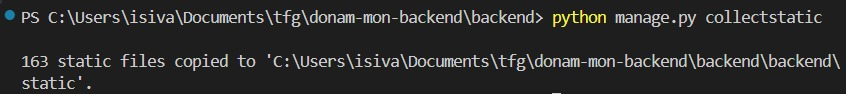
\includegraphics[width=0.9\textwidth]{figs/back.jpg}
    \caption{Recopilación de archivos estáticos con \texttt{collectstatic} en Django}
\end{figure}

\subsection{Gestión de geolocalización y decisión sobre campos GIS}

Aunque el proyecto tiene incluida la librería \texttt{djangorestframework-gis} (puedes verla en el archivo \texttt{requirements.txt}), en realidad no se está usando porque no se han definido campos GIS como \texttt{PointField} o \texttt{PolygonField}, ni tampoco se utiliza el backend geoespacial de Django (\texttt{django.contrib.gis.db.backends.postgis}).

Para la geolocalización, simplemente se guardan las coordenadas de latitud y longitud como campos \texttt{FloatField} en el modelo \texttt{Lugar}:

\begin{lstlisting}[language=Python, caption={Fragmento del modelo Lugar}]
class Lugar(models.Model):
    nombre = models.CharField(max_length=100)
    descripcion = models.TextField()
    latitud = models.FloatField(blank=True, null=True)
    longitud = models.FloatField(blank=True, null=True)
    # ...otros campos...
\end{lstlisting}

Esta solución es suficiente para lo que necesita la aplicación ahora mismo: permite guardar y consultar posiciones geográficas sin complicaciones y sin depender de librerías adicionales ni configuraciones avanzadas. Además, facilita la integración y el despliegue usando el backend estándar de PostgreSQL (\texttt{django.db.backends.postgresql}), sin tener que recurrir a PostGIS.

\textbf{Ventajas de este enfoque:}
\begin{itemize}
    \item El modelo de datos es más sencillo y fácil de mantener.
    \item La integración y el despliegue funcionan en cualquier entorno PostgreSQL, sin requisitos especiales.
    \item Se evitan dependencias y configuraciones extra.
\end{itemize}

En una posible evolución, si en algún momento se necesitan consultas espaciales más avanzadas o funcionalidades GIS (por ejemplo, búsquedas por proximidad o rutas optimizadas), se podría migrar a campos GIS y aprovechar tanto PostGIS como \mbox{\texttt{djangorestframework-gis}} sin demasiada dificultad.
\section{Implementación del frontend}

\subsection{Herramientas, frameworks y lenguajes utilizados}

El frontend de la aplicación se ha desarrollado utilizando el framework \textbf{React Native} para asegurar la compatibilidad multiplataforma (Android, iOS y web). Se ha utilizado \textbf{Expo} para simplificar el desarrollo, pruebas y despliegue, así como para acceder a funcionalidades nativas como la cámara, la geolocalización y las notificaciones.

Las principales herramientas y librerías utilizadas son:
\begin{itemize}
    \item \textbf{React Native} (v0.79.2)
    \item \textbf{Expo} (v53.0.9)
    \item \textbf{React Navigation} para la gestión de la navegación entre pantallas
    \item \texttt{@react-native-async-storage/async-storage} para almacenamiento local seguro
    \item \texttt{axios} para peticiones HTTP
    \item \texttt{expo-location} y \texttt{expo-notifications} para geolocalización y notificaciones push
    \item \texttt{react-native-maps} para mostrar mapas y marcadores
    \item \texttt{react-native-vector-icons} para iconografía
    \item \texttt{expo-camera} para escaneo de QR en rutas
    \item \texttt{@react-native-picker/picker} para selectores personalizados
\end{itemize}

\subsection{Estructura del proyecto y organización del código}

El código fuente del frontend se encuentra en la carpeta \texttt{donam-mon-frontend/my-app/}, que contiene los componentes, utilidades, estilos y recursos gráficos. La estructura principal es la siguiente:

\begin{lstlisting}[language=bash, caption={Estructura principal del frontend}]
my-app/
    App.js
    apiConfig.js
    index.js
    assets/
        # Imágenes y recursos gráficos
        ...
    Donammon/
        Main.js
        Mapa.js
        Mujeres.js
        PerfilUsuario.js
        Detail.js
        RutaDetail.js
        HistorialLugares.js
        HistorialRutas.js
        NotificacionProximidad.js
        AR.js
        Filtros.js
        FiltrosContext.js
        Login.js
        Register.js
        Welcome.js
        NavigationApp.js
        Rutas.js
        ...
    styles/
        styles.js
        styles-detail.js
        styles-filtros.js
        styles-perfil.js
        ...
\end{lstlisting}

\texttt{App.js}: Punto de entrada principal, configura el proveedor de filtros y la navegación.

\texttt{Donammon/}: Carpeta principal de componentes de pantalla y utilidades.

\texttt{assets/}: Imágenes y recursos gráficos usados en la interfaz.

\subsection{Navegación y estructura de pantallas}

La navegación principal se gestiona mediante un \textbf{Bottom Tab Navigator} definido en \texttt{Main.js}, que organiza la aplicación en pestañas: Mapa, Mujeres, Rutas, Realidad Aumentada (RA) y Perfil.

\begin{lstlisting}[language=, caption={Definición de pestañas en Main.js}]
<Tab.Navigator
    screenOptions={{
        tabBarActiveTintColor: '#5f68c4',
        tabBarInactiveTintColor: '#000000',
        tabBarStyle: { backgroundColor: '#edebff' },
    }}
>
    <Tab.Screen 
        name="Mapa" 
        component={Mapa} 
        initialParams={route.params} 
        options={{ 
            headerShown: false,
            tabBarIcon: ({ color, size }) => (
                <Image source={require('../assets/mapa.png')} />
            ),
        }} 
    />
    <Tab.Screen name="Mujeres" component={MujeresCombinadas} ... />
    <Tab.Screen name="Rutas" component={Rutas} ... />
    <Tab.Screen name="RA" component={AR} ... />
    <Tab.Screen name="Perfil" component={PerfilUsuario} ... />
</Tab.Navigator>
\end{lstlisting}

Cada pantalla principal se implementa como un componente independiente, facilitando la escalabilidad y el mantenimiento.

Además, la navegación global de la app se gestiona mediante un \textbf{Stack Navigator} definido en \texttt{NavigationApp.js}, que permite acceder a pantallas como el login, registro, detalle de lugar, historial de visitas o filtros, además de la pantalla principal con pestañas. El componente \texttt{App.js} monta el contexto global de filtros y notificaciones, y envuelve toda la navegación de la aplicación.
\subsection{Gestión de usuarios y autenticación}

La autenticación de usuarios se realiza mediante peticiones a la API del backend. El login y el registro almacenan el token de autenticación en \texttt{AsyncStorage} para su uso en futuras peticiones.

\begin{lstlisting}[language=, caption={Ejemplo de login en Login.js}]
const validateLogin = async () => {
    try {
        const response = await fetch('http://192.168.1.44:8000/api/api-token-auth/', {
            method: 'POST',
            headers: { 'Content-Type': 'application/json' },
            body: JSON.stringify({ username, password }),
        });
        if (response.ok) {
            const data = await response.json();
            await AsyncStorage.setItem('token', data.token);
            navigation.navigate('Main');
        } else {
            Alert.alert('Error', 'Usuario o contraseña incorrectos');
        }
    } catch (error) {
        Alert.alert('Error', 'No se pudo conectar con el servidor');
    }
};
\end{lstlisting}

El perfil de usuario permite cambiar el nombre de usuario y cerrar sesión, eliminando el token almacenado.

\subsection{Visualización de mujeres y lugares}

La pantalla \texttt{Mujeres.js} muestra una lista de lugares destacados asociados a mujeres relevantes, permitiendo filtrar por área, visitados y búsqueda por nombre.

\begin{lstlisting}[language=, caption={Filtrado y renderizado de lugares}]
const filteredLugares = allLugares
    .filter(lugar => selectedSection === 'Todas' || lugar.area === selectedSection)
    .filter(lugar => selectedVisited === 'Todas' || (selectedVisited === 'Visitadas' ? lugar.visited : !lugar.visited))
    .filter(lugar => !searchTerm || lugar.nombre.toLowerCase().includes(searchTerm.toLowerCase()));
\end{lstlisting}

Cada tarjeta de lugar muestra la imagen, nombre, área, distancia y estado de visita, y permite acceder al detalle.

\subsection{Detalle de lugar y gestión de visitas}

La pantalla \texttt{Detail.js} muestra la información completa de un lugar, incluyendo la mujer asociada, descripción, dirección, fechas, imagen y estado de visita. Permite marcar el lugar como visitado o no visitado, sincronizando el estado con el backend mediante una petición HTTP autenticada. Además, la pantalla ofrece funcionalidades avanzadas para mejorar la experiencia del usuario:

\begin{itemize}
    \item \textbf{Compartir información del lugar:} El usuario puede compartir el lugar y su imagen a través de las opciones nativas del dispositivo. Se genera un mensaje con los datos relevantes y, si existe, se adjunta la imagen descargada temporalmente.
    \item \textbf{Visualización de imágenes ampliadas:} Al pulsar sobre la imagen de la mujer o del lugar, se muestra la imagen en grande en un modal.
    \item \textbf{Visualización de información enriquecida:} Se muestran áreas de investigación como chips, fechas, ámbito, descripción, dirección, un mapa con la localización exacta y la distancia al usuario.
\end{itemize}

A continuación se muestra un ejemplo de la función para marcar un lugar como visitado o no visitado:

\begin{lstlisting}[language=, caption={Marcar como visitado}]
const toggleVisited = async () => {
    const updatedLugar = { ...lugar, visited: !lugar.visited };
    navigation.setParams({ lugar: updatedLugar });
    const token = await AsyncStorage.getItem('token');
    if (!token) return;
    if (!lugar.visited) {
        // Marcar como visitado
        try {
            const response = await fetch('http://192.168.1.44:8000/api/visit-lugar/', {
                method: 'POST',
                headers: { 'Content-Type': 'application/json', 'Authorization': `Token ${token}` },
                body: JSON.stringify({ lugar_id: lugar.id }),
            });
            const data = await response.json().catch(() => ({}));
            if (!response.ok) {
                throw new Error(`Error ${response.status}: ${JSON.stringify(data)}`);
            }
        } catch (error) {
            console.error('Error registrando visita:', error);
        }
    } else {
        // Marcar como no visitado (eliminar del historial)
        try {
            await fetch('http://192.168.1.44:8000/api/visited-lugares/', {
                method: 'PUT',
                headers: { 'Content-Type': 'application/json', 'Authorization': `Token ${token}` },
                body: JSON.stringify({ lugar_id: lugar.id }),
            });
        } catch (error) {
            console.error('Error eliminando visita:', error);
        }
    }
};
\end{lstlisting}

Y la función para compartir la información del lugar:

\begin{lstlisting}[language=, caption={Función para compartir la información del lugar}]
const compartirLugar = async () => {
    try {
        let message = "Echa un vistazo a este lugar de la aplicación Dona'm Món!\n\n";
        message += `Nombre del lugar: ${lugar.nombre}\n`;
        if (lugar.mujer_nombre) message += `Mujer destacada: ${lugar.mujer_nombre}\n`;
        if (lugar.mujer_descripcion) message += `Sobre ella: ${lugar.mujer_descripcion}\n`;
        if (lugar.direccion) message += `Dirección: ${lugar.direccion}\n`;
        if (lugar.descripcion) message += `Descripción: ${lugar.descripcion}\n`;
        let options = { message };
        if (lugar.foto) {
            // Descargar la imagen a un archivo temporal
            const fileUri = FileSystem.cacheDirectory + 'lugar.jpg';
            const downloadRes = await FileSystem.downloadAsync(lugar.foto, fileUri);
            if (downloadRes.status === 200) {
                options = { ...options, url: downloadRes.uri };
            }
        }
        await Share.share(options);
    } catch (error) {
        console.error('Error al compartir el lugar:', error);
    }
};
\end{lstlisting}


\subsection{Mapas y geolocalización}

La pantalla \texttt{Mapa.js} utiliza \texttt{react-native-maps} para mostrar todos los lugares en un mapa, con iconos personalizados y colores según el estado de visita. Permite filtrar lugares y ver detalles al pulsar sobre un marcador.

\begin{lstlisting}[language=, caption={Marcadores en el mapa}]
<MapView>
    {filteredLugares.map(lugar => (
        <Marker
            key={lugar.id}
            coordinate={{ latitude: lugar.latitud, longitude: lugar.longitud }}
            pinColor={lugar.visited ? '#43a047' : '#5f68c4'}
        >
            <Callout>
                <Text>{lugar.nombre}</Text>
                <Text>{lugar.mujer_nombre}</Text>
            </Callout>
        </Marker>
    ))}
</MapView>
\end{lstlisting}

La ubicación del usuario se obtiene con \texttt{expo-location}, permitiendo calcular distancias y mostrar solo lugares cercanos si se desea.

\subsection{Gestión de rutas temáticas}

La pantalla \texttt{Rutas.js} y \texttt{RutaDetail.js} permiten visualizar rutas temáticas, ver los lugares que las componen y marcar cada lugar como visitado mediante escaneo de QR. El progreso de la ruta se muestra visualmente y se puede reiniciar la ruta si se desea.

\begin{lstlisting}[language=, caption={Escaneo de QR y registro de visita}]
const handleBarcodeScanned = async ({ data }) => {
    const lugar = ruta.lugares.find(l => l.nombre.toLowerCase() === data.toLowerCase());
    if (lugar) {
        await fetch('http://192.168.1.44:8000/api/visit-lugar-ruta/', {
            method: 'POST',
            headers: { 'Content-Type': 'application/json', 'Authorization': `Token ${token}` },
            body: JSON.stringify({ ruta_id: ruta.id, lugar_id: lugar.id }),
        });
        setScanMsg('Lugar de ruta marcado como visitado!');
        await fetchVisitedRuta();
    } else {
        setScanMsg('QR no corresponde a ningun lugar de la ruta.');
    }
};
\end{lstlisting}

\subsection{Historial de lugares y rutas visitadas}

Las pantallas \texttt{HistorialLugares.js} y \texttt{HistorialRutas.js} muestran el historial de lugares y rutas visitadas por el usuario, permitiendo borrar el historial si se desea.

\begin{lstlisting}[language=, caption={Borrado de historial de rutas}]
const handleClearHistory = async () => {
    const token = await AsyncStorage.getItem('token');
    for (const ruta of rutasCompletadas) {
        await fetch(`http://192.168.1.44:8000/api/visited-lugares-ruta/?ruta_id=${ruta.id}`, {
            method: 'DELETE',
            headers: { 'Authorization': `Token ${token}` },
        });
    }
    setRutasCompletadas([]);
    Alert.alert('Éxito', 'Historial de rutas completadas borrado.');
};
\end{lstlisting}

\subsection{Notificaciones y proximidad}

La app utiliza \texttt{expo-notifications} y \texttt{expo-location} para enviar notificaciones cuando el usuario se acerca a un lugar destacado. El componente \texttt{NotificacionProximidad.js} gestiona esta lógica, comprobando la distancia a los lugares y mostrando alertas contextuales.

\begin{lstlisting}[language=, caption={Notificación de proximidad}]
if (dist !== null && dist <= 3 && !notifiedIds.current.has(lugar.id)) {
    await Notifications.scheduleNotificationAsync({
        content: {
            title: 'Estas cerca de un lugar destacado!',
            body: `Te encuentras a ${dist.toFixed(2)} km de ${lugar.nombre} (${lugar.mujer_nombre})`,
        },
        trigger: null,
    });
    notifiedIds.current.add(lugar.id);
}
\end{lstlisting}

\subsection{Realidad aumentada}

La pantalla \texttt{AR.js} permite acceder a experiencias de realidad aumentada asociadas a ciertos lugares, abriendo el visor web correspondiente si el usuario está cerca del lugar.

\begin{lstlisting}[language=, caption={Acceso a AR}]
if (distance <= 3) {
    openURL(lugar.ar_url);
}
\end{lstlisting}

\subsection{Gestión de estilos y diseño}

Los estilos se gestionan en archivos como \texttt{styles.js} y \texttt{styles-perfil.js}, utilizando \texttt{StyleSheet} de React Native para mantener la coherencia visual y facilitar la personalización.

\begin{lstlisting}[language=, caption={Ejemplo de estilos en styles.js}]
const styles = StyleSheet.create({
    container: {
        flex: 1,
        backgroundColor: '#f9efe8',
        alignItems: 'center',
        justifyContent: 'center',
    },
    filterButton: {
        backgroundColor: '#7196e4',
        paddingVertical: 0,
        paddingHorizontal: 30,
        borderRadius: 10,
        marginTop: 23,
        alignSelf: 'center',
        width: width + 20,
        height: 39,
        alignItems: 'center',
    },
    // otros estilos...
});
\end{lstlisting}

\subsection{Gestión de almacenamiento local}

Se utiliza \texttt{AsyncStorage} para guardar el token de usuario, preferencias y otros datos persistentes, asegurando que la sesión se mantenga entre reinicios de la app.

\begin{lstlisting}[language=, caption={Uso de AsyncStorage}]
await AsyncStorage.setItem('token', data.token);
const token = await AsyncStorage.getItem('token');
\end{lstlisting}

\subsection{Integración con la API y manejo de errores}

Todas las peticiones a la API del backend se realizan mediante \texttt{fetch} o \texttt{axios}, gestionando los errores y mostrando mensajes claros al usuario en caso de fallo.

\begin{lstlisting}[language=, caption={Manejo de errores en peticiones}]
try {
    const response = await fetch('http://192.168.1.44:8000/api/visited-lugares/', { /* ... */ });
    if (!response.ok) throw new Error('Error al cargar lugares visitados');
    const data = await response.json();
    setVisitedCount(data.length);
} catch (error) {
    Alert.alert('Error', 'No se pudo cargar el historial');
}
\end{lstlisting}

\subsection{Pruebas y depuración}

Durante el desarrollo, se han utilizado logs en consola y mensajes de alerta para depurar la lógica de la app y asegurar el correcto funcionamiento de todas las funcionalidades.

\begin{lstlisting}[language=, caption={Ejemplo de logs y alertas}]
console.log('Detalle lugar:', lugar);
Alert.alert('Éxito', 'Nombre de usuario actualizado');
\end{lstlisting}
